\chapter{Interesting results}
\section{Implementation}
Referring back to Figure \ref{fig:my_label}. We can then implement the iteration of matrix $M$ by employing the function $F(M,\alpha)$ that encodes the rules of the simulation. The way it iterates is While $k\leq600$:\par
$$M_{k+1}=F(M_{k}, \alpha)$$ 
$$G_{k}=f(M_{k})$$
$$H_{k}=\sum XOR(G_{k})$$
Where f just flattens the matrix $M$. Now, the task is to display $M_{k+1}$ and plot 600 points of $(k, E_{k})$ side by side. A potential way to look at how the heat conduction analog, $\alpha$ affects the final entropy after 600 iterations are to check $H_{600}$ for different $\alpha$ values. Some of the static images of the effect of $\alpha$ are shown in Figure \ref{fig: grid_600}.  
   \begin{figure}[H]
        \centering
        \begin{subfigure}[b]{0.475\textwidth}
            \centering
        \includegraphics[width=4.5cm,height=4.5cm]{images/image0.png}
            \caption[The initial grid]%
            {{\small The initial grid}}    
            \label{fig:input_0}
        \end{subfigure}
        \hfill
        \begin{subfigure}[b]{0.475\textwidth}  
            \centering 
            \includegraphics[width=4.5cm,height=4.5
            cm]{images/image1.png}
            \caption[$\alpha=10\%$]%
            {{\small $\alpha=10\%$}}    
            \label{fig:output_10}
        \end{subfigure}
        \vskip\baselineskip
        \begin{subfigure}[b]{0.475\textwidth}   
            \centering 
            \includegraphics[width=4.5cm,height=4.5cm]{images/image2.png}
            \caption[$\alpha=40\%$]%
            {{\small $\alpha=40\%$}}    
            \label{fig:output_40}
        \end{subfigure}
        \hfill
        \begin{subfigure}[b]{0.475\textwidth}   
            \centering 
            \includegraphics[width=4.5cm,height=4.5cm]{images/image3.png}
            \caption[$\alpha=100\%$]%
            {{\small $\alpha=100\%$}}    
            \label{fig:output_100}
        \end{subfigure}
        \caption[ The average and standard deviation of critical parameters ]
        {\small The Grid after 600 iterations } 
        \label{fig: grid_600}
    \end{figure}
The grid is a 250x250 matrix where $E=2438$. The initial grid $M_{1}$ is Figure \ref{fig:input_0} which is a large rectangular box. Activated cells (1) are colored yellow while the other cells (0) are colored black. As seen from the figures, it can be seen that $\alpha$ has a large effect on how spread out the activated cells are. \par

\vspace{0,3cm}
The general effects of $\alpha$ on the proxy entropy measurement $H$ can be seen on Figure \ref{fig:H_1000} shown below: 
\begin{figure}[H]
    \centering
    \includegraphics[width=10cm,height=8cm]{images/Entropy_data.png}
    \caption{The effects of $\alpha$ on the final entropy after set amount of simulations}
    \label{fig:H_1000}
\end{figure}
The above figure runs have 20 different points for $\alpha$ (Move probability) ranging from 0 to 1 in increments of 0.05. For each of these points, 5 simulations were run and the arithmetic means of these 5 simulations of 300,600, and 1000 iterations were collected. The final points that are associated with the $\alpha$ are then plotted for 300, 600, and 1000 iterations. Here the Matrix $M$ is a standardized square matrix of 250x250 with an E value of 2438. \par

\vspace{0.3cm}
As seen from Figure \ref{fig:H_1000} the graph shows that $\alpha$ has a tremendous effect on the final proxy entropy $H$, with diminishing returns. A similar trend of increasing $H$ followed by a decrease in the gradient of the graph is seen in Figure \ref{fig:normal} \par

\vspace{0.3cm}
For Figure \ref{fig:normal}, the simulation's proxy entropy $H$ is plotted against its iteration. For $\alpha=1$, $H$ shows a sharp increase in the first few iterations and the gradient of the graph decreases over the iterations. The trend indicates that maximum entropy will be reached when the iteration number becomes very large. While the graph trends upwards, there are slight variations for $H$. This is because the random nature of the simulation might decrease the number of unique occurrences of $(1,0), (0,1)$. However, the number of unique alternative $(1,0), (0,1)$ will increase as the underlying matrix gets more homogeneous simply because many more configurations match a homogeneous distribution rather than an ordered structure. \par
\begin{figure}[H]
     \centering
     \begin{subfigure}[H]{0.6\textwidth}
         \includegraphics[width=10cm,height=5.5cm]{images/im1.png}
         \caption{$\alpha=0.2$}
         \label{fig:res_1}
     \end{subfigure}
      \vskip\baselineskip
     \begin{subfigure}[H]{0.6\textwidth}
         \includegraphics[width=10cm,height=5.5cm]{images/im2.png}
         \caption{$\alpha=1$}
         \label{fig:res_2}
     \end{subfigure}
        \caption{Results after 600 iterations for different alpha values}
        \label{fig:normal}
\end{figure}
\subsection{Known Bugs}
From Figure \ref{fig:output_100}, it is visible that the colored cells tend to go up. Investigating further reveals that there might be a bug within the implementation of $F(M,\alpha)$. 
We can investigate the problem further by identifying which directions the code chooses. There are 8 pairs of directions it can choose, these are: 
$$([0, -1],[-1, 0], [1, 0], [0, 1], [-1, -1], [1, -1], [1, 1], [-1, 1])$$
We can mark these directions into an appropriate string, such as: $$["T","L","R","B","TL","TR","BR","BL"]$$ 
Each corresponds to the pairs. In this case, T is top direction L is left, R is right, TL is top-left and BL is bottom right. Finally, we can run a while loop for 6000 iterations and plot the results on a histogram to see which letter it chooses the most. \par

\vspace{0.3cm}
In Figure \ref{fig:bias} it can be seen that the string "T", associated with the direction vector $[0, -1]$ is chosen slightly more than the rest, with a rate of 13.5\%. The differences are small but they are noticeable as in Figure \ref{fig:output_100}, the colored points tend to go slightly upwards. As for the current situation, I have yet to know what is causing this slight drift within the directions. \par
\begin{figure}[H]
    \centering
    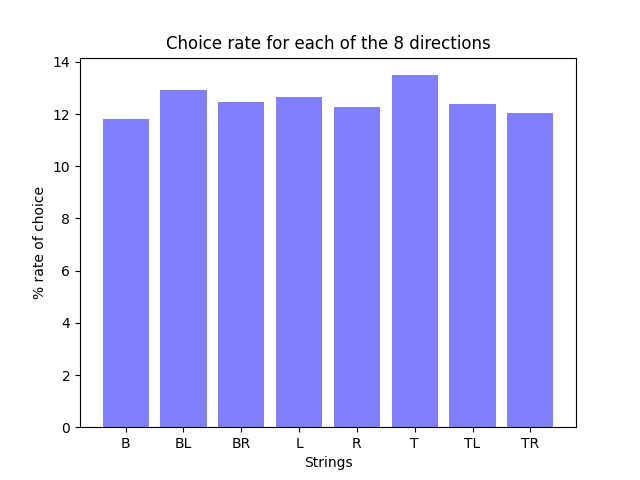
\includegraphics[width=10cm,height=7.5cm]{images/bias.png}
    \caption{Frequency density of the 8 possible directions after 6000 iterations}
    \label{fig:bias}
\end{figure}
\subsection{Further plans for Version 2}
In Quantum mechanics, certain discrete energy levels are allowed. Such a system is usually depicted in Figure \ref{fig:e_levels} below: 
\begin{figure}[H]
    \centering
    \includegraphics[width=4cm,height=5cm]{images/E_levels.png}
    \caption{Discrete energy levels}
    \label{fig:e_levels}
\end{figure}
The level corresponding to "e" is the ground state or the lowest energy state that a particle can carry. This hypothetical particle can take up to 5e units of energy. \par

\vspace{0.3cm}
Things get interesting when one questions how many different energy levels are possible when there are 2 or more particles involved with a set energy level. Defining $E$ is the total amount of energy as before, we can count the total amount of energy for 2 particles to be $e_{1}+e_{2}$. Our job is to then find the total number of integer combinations where $e_{1},e_{2} \ge 1$, and both of them add up to $E$. If E=4 then there are 3 pairs of $e_{1}$ and $e_{2}$. These are $(1,3), (3,1), (2,2) $ which corresponds to 3 different micro-states. To see how more particles affect the different number of combinations you can view a \href{https://www.youtube.com/watch?v=mg0hueOyoAw}{video} made by Parth G in which he does a really good job in explaining what is happening. \par

\vspace{0.3cm}
Going back to the rules, which are: 
\begin{itemize}
    \item \textbf{Law 1: }A cell can either be a 1 or a 0, on or off.
    \item \textbf{Law 2: }The number of 1s ($E$) within the Matrix M cannot change.
    \item \textbf{Law 3: }Each of the 1s can move to an empty square (0) that is 1 square surrounding it.
    \item \textbf{Features: }There is a probability multiplier labeled $\alpha$ which modifies the chances of "heat transfer". Generally, this can be read that if it can move it will move, if it can't it won't. 
\end{itemize}
I wondered what if I modified Law 1 while keeping everything else constant. What if Law 1 is restated as: 
\begin{itemize}
    \item \textbf{Law 1: }A cell can take up to 9 energy levels with the ground state corresponding to 0 and the maximum energy corresponding to 8.
\end{itemize}
This means that each of the cells at Matrix $M$ can only take integer values of $0,1,2,3,4,5,6,7,8$ while the rules of heat transfer are still governed. Meaning that any cell that is less than 8 is a vacant cell in which energy can transfer. \par

\vspace{0.3cm}
Such a change within the rules would be interesting to simulate. However, entropy will be quite a problem to recompute. In version 1 of Automata, Entropy was simply calculated by applying the XOR function to a flattened matrix $M$ called matrix $G$. I could make an array of truth values such that any value bigger than 0 will be captured as 1 and that counting unique occurrences of $(1,0), (0,1)$ would reveal how spread out the energy is. Following that, a spread-out configuration corresponds to more micro-states which means higher entropy. \par

\vspace{0.3cm}
While this could work, such a technique is ridden with problems and will require a lot more thought to reformulate. Alas, more research would need to be conducted and a careful approach to picking a solution matched to my problem would need to be adopted. 
